\newsection

\subsection{BP 9:
 Okushiri Island (Field)}

{\bf Documentation:}
\begin{itemize} 
\item PMEL-135, pp 8 \& 48-53 \cite{SynolakisBernard:pmel135}.
\item A problem description is provided by Frank Gonz\'alez 
 at \cite{bp-description}:\\
\href{https://github.com/rjleveque/nthmp-benchmark-problems/blob/master/BP09-FrankG-Okushiri\_island/Description.pdf} 
{BP09-FrankG-Okushiri\_island/Description.pdf} 
\item Numerous other publications also describe this event, in varying detail: 
\cite{DCRC1994,HTSG1993,KatoTsuji1994,TakahashiEtAl1995,Takahashi1996}
\end{itemize} 

\subsubsection{Description}
The goal of this Benchmark Problem (BP) is to compare computed model results with field observations of the 1993 Okushiri Island tsunami.

\subsubsection {Problems encountered}

\begin {itemize}
\item The primary problem encountered was the uncertain quality of the computational bathymetric topographic grids. 

\end{itemize} 

\subsubsection{What we did}

\begin{itemize}
\item Used g = 9.81 and no friction.
\item Used bathy/topo grids and source grid for the Disaster Control Research Center solution DCRC17a.  Dmitry Nicolsky provided improved versions of the originals developed by Kansai University, in which severe misalignments in the original data were reduced.  The computational domain and initial conditions imposed by the source deformation are presented in Figure \ref{DomainSource}
\end{itemize}

\begin{figure}[ht]
\hfil\includegraphics[width=6.0in]{bp9/DomainSource.png}\hfil
\caption{\label{DomainSource}
Computational domain and source deformation.
  }
\end{figure} 

\subsubsection{Problem Requirements}
  Requirements of this benchmark test were to:
\begin{enumerate}
\item  Compute runup around Aonae
\item  Compute arrival of the first wave to Aonae
\item  Show two waves at Aonae approximately 10 min apart; the first wave came from the west, the second wave came from the east
\item  Compute water level at Iwanai and Esashi tide gauges
\item  Maximum modeled runup distribution around Okushiri Island
\item  Modeled runup height at Hamatsumae
\item  Modeled runup height at a valley north of Monai
\end{enumerate}

\subsubsection{Results}

Figures \ref{bp9full} through  \ref{bp9aonae} shows results of one computation where AMR is used to concentrate grid points near the southern Aonae Peninsula. The rectangular boxes show regions of refinement.  The coarsest grid is a $60\times 60$ grid on a 1-degree square as shown in Figure \ref{bp9full}. Five levels of refinement are used going down by factors 2, 4, 4, and 6 from each level to the next. In this computation, Level 4 is only allowed on the southern half of Okushiri Island and Level 5 only around the Aonae Peninsula. 

Figure \ref{bp9ok} shows a zoom on the island and Figure \ref{bp9aonae} a further zoom on the peninsula. 
Arrival of the first wave at Aonae (Requirement 2) is seen from the west at about $t = 5$ minutes.  The second major wave arrives from the east at about 10 minutes.    

Figure \ref{bp9inaonae} shows the inundation level on the peninsula.  The color scale indicates the maximum depth of water ever recorded at each point on a fixed grid that is placed around this region.  




 % the subsequrent runup around Aonae (Requirement 1) is presented in Figure \ref{AonaeRunup}.  The first wave arrived at about t = 5 minutes, and wrapped around the peninsula, engulfing Aonae proper in about 2 minutes, at t = 7 minutes, as seen in Figure \ref{Aonae07min.png}.  Between 9 and 10 minutes later, at t=16 and 17 minutes, Hamatsumae (\ref{Aonae16min.png} and then the northeastern coast of the Aonae peninsula \ref{Aonae17min.png} are inundated by a wave from the east (Requirements 3 and 6).  Figures \ref{WestObsVsGeoClaw} and \ref{EastObsVsGeoClaw} present the observed and modeled maximum runup distribution on the West and East coasts of Okushiri, respectively (Requirement 5), including a valley north of Monai where the observed runup height that exceeded 30 m \ref{WestObsVsGeoClaw} (Requirement 7).  Figures \ref{Iwanai} and \ref{Esashi} present the model results and tide gage time series at Iwanai and Esashi.  The correspondence of model and observed tides is poor at both locations, perhaps due to the issue of inaccurate spatial registration of the tide gage positions and the corresponding computational grid cell.  

 
Figure \ref{bp9TeamStations} shows the runup at various other points around the island as measured by the team of Y. Tsuji, along with values computed using GeoClaw.  Figure \ref{bp9scatter} shows a scatter plot of the correlation between the observations and the computed values.  The GeoClaw values were obtained by placing a small fixed grid around each observation point and recording the maximum water depth at each point on this grid at each timestep of the computation, using built-in feature of GeoClaw.  The maximum depth over time can also be accumulated at these points and updated each time step.  Plots of the maxima over these grids gives a visualization of the maximum extent of inundation.  Such plots are shown  in Figures \ref{bp9inaonae} and \ref{bp9monai}, with 4-meter contours.  For most other observation  points contours of topography at 2-meter increments were plotted in order to better estimate the maximum runup in a small region centered about each observation point. 
%Figure \ref{bp9fg} shows a sample of several of these inundation maps. 

Figure \ref{bp9monai} shows the inundation map for the Monai Valley, with 4-meter contour lines.  Inundation to roughly 32 m is observed, in accordance with observations.

Computed arrival times agree well with eye-witness observations at Aonae and Hamatsumae, and computed runup values agree reasonably well with observed values (Figure \ref{WestObsVsGeoClaw}).  

\ignore{
\begin{figure}[ht]
\hfil\includegraphics[width=5.0in]{bp9/AonaeFirstWave.png}\hfil
\caption{\label{AonaeFirstWave}
First wave arrival at Aonae.
  }
\end{figure} 

\begin{figure}[ht]
\hfil\includegraphics[width=5.0in]{bp9/Aonae07min.png}\hfil
\caption{\label{Aonae07min}
Runup at Aonae.
  }
\end{figure}

\begin{figure}[ht]
\hfil\includegraphics[width=5.0in]{bp9/Aonae16min.png}\hfil
\caption{\label{Aonae16min}
Second wave from the east begins to inundate Hamatsumae and the northeastern coast of the Aonae peninsula.
  }
\end{figure} 

\begin{figure}[ht]
\hfil\includegraphics[width=5.0in]{bp9/Aonae17min.png}\hfil
\caption{\label{Aonae17min}
Runup at Hamatsumae and the northeastern coast of the Aonae peninsula.
  }
\end{figure} 

\begin{figure}[ht]
\hfil\includegraphics[width=5.0in]{bp9/WestObsVsGeoClaw.pdf}\hfil
\caption{\label{WestObsVsGeoClaw}
Observed and modeled maximum runup on the Okushiri West Coast.
  }
\end{figure} 

\begin{figure}[ht]
\hfil\includegraphics[width=5.0in]{bp9/EastObsVsGeoClaw.pdf}\hfil
\caption{\label{EastObsVsGeoClaw}
Observed and modeled maximum runup on the Okushiri East Coast.
  }
\end{figure} 
}

%-------------

\begin{figure}[ht]
\hfil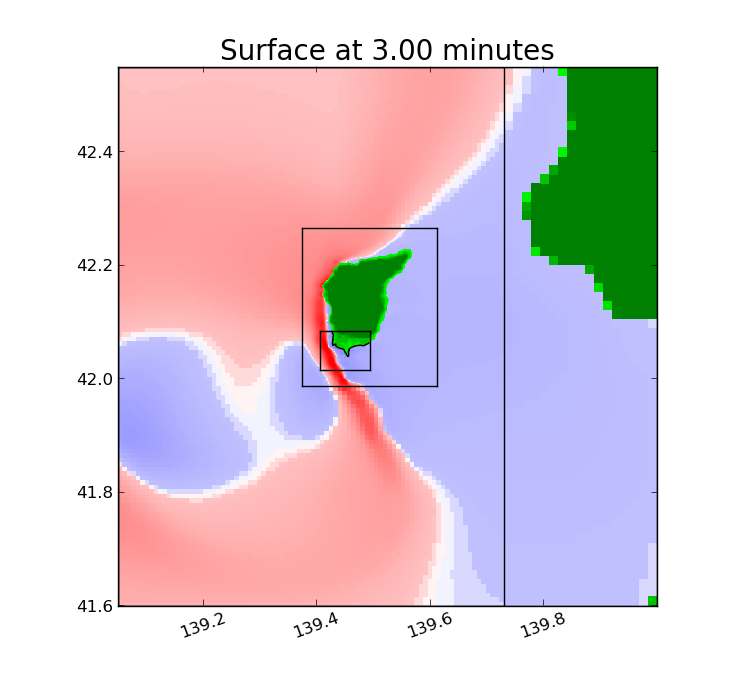
\includegraphics[width=2.8in]{bp9/full_3min.png}\hfil
\hfil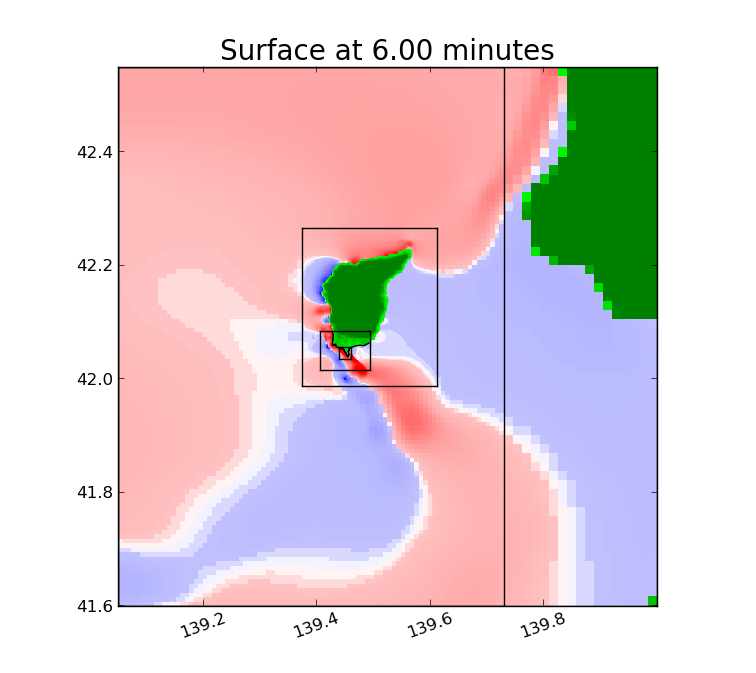
\includegraphics[width=2.8in]{bp9/full_6min.png}\hfil

\caption{\label{bp9full}
Full computational domain for one simulation, in which AMR grids are focused near the Aonae Peninsula at the south of Okushiri Island.
  }
\end{figure}

\begin{figure}[ht]
\hfil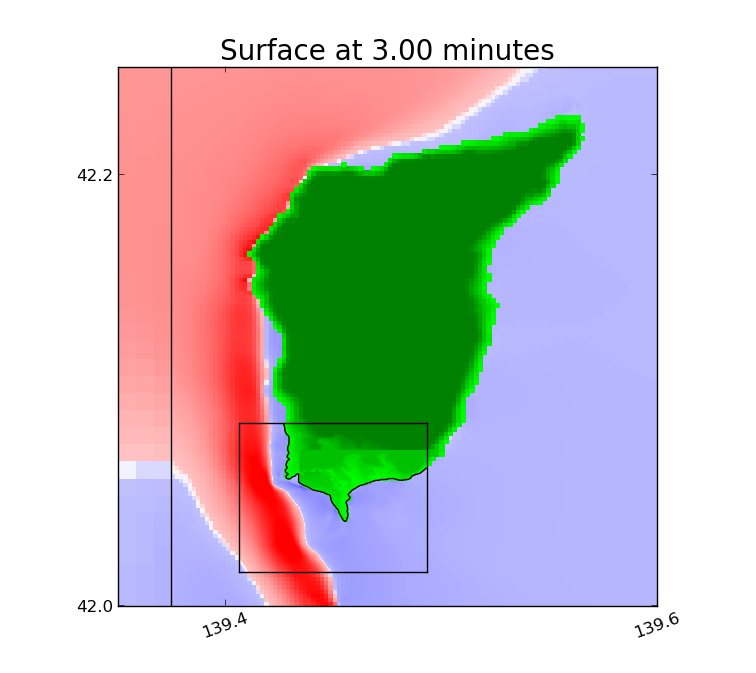
\includegraphics[width=2.0in]{bp9/ok_3min.png}\hfil
\hfil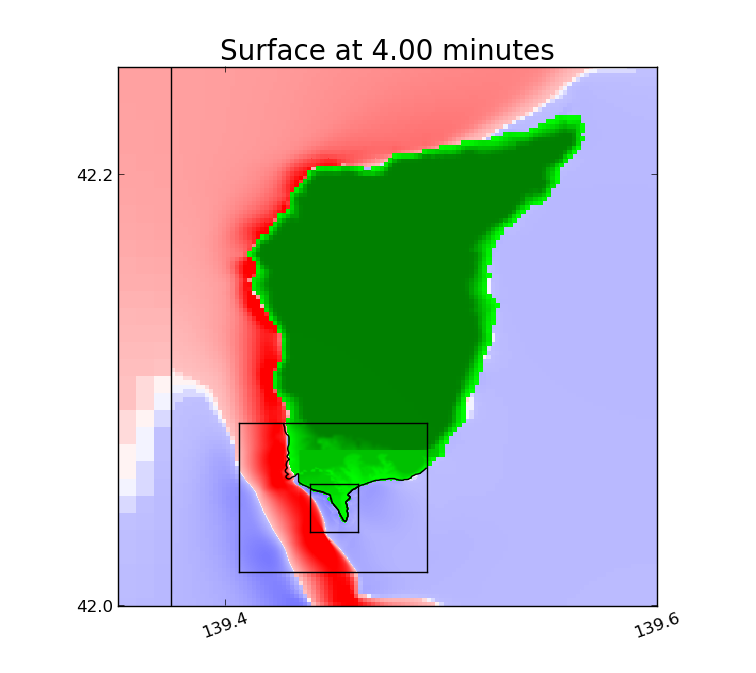
\includegraphics[width=2.0in]{bp9/ok_4min.png}\hfil
\hfil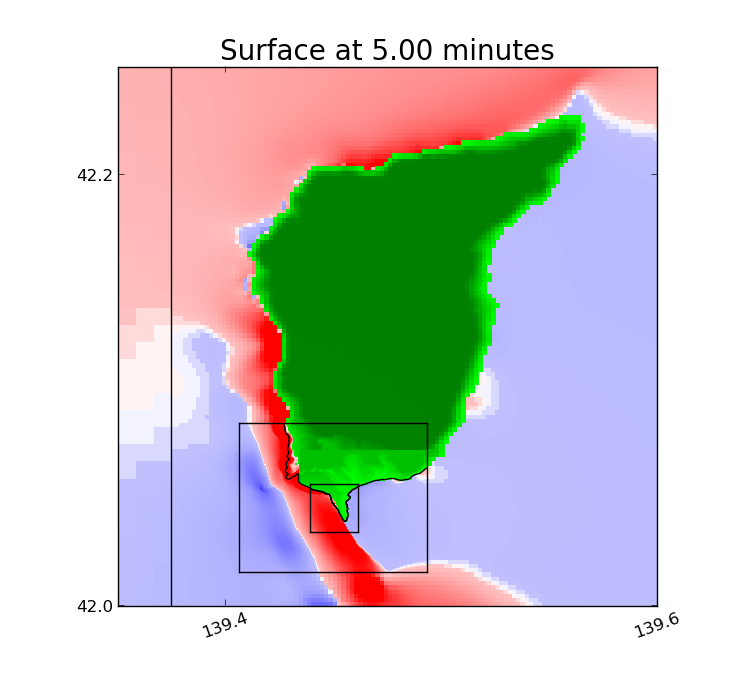
\includegraphics[width=2.0in]{bp9/ok_5min.png}\hfil
\vskip 10pt
\hfil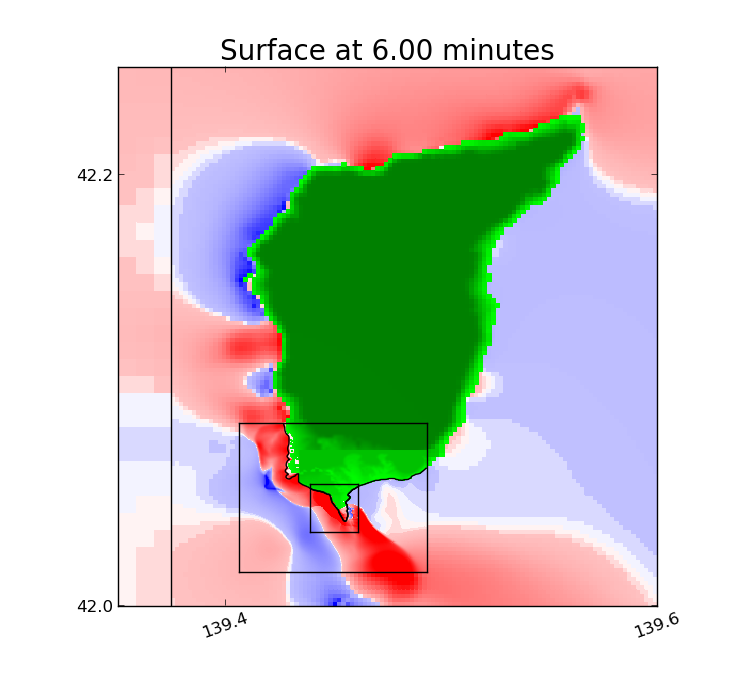
\includegraphics[width=2.0in]{bp9/ok_6min.png}\hfil
\hfil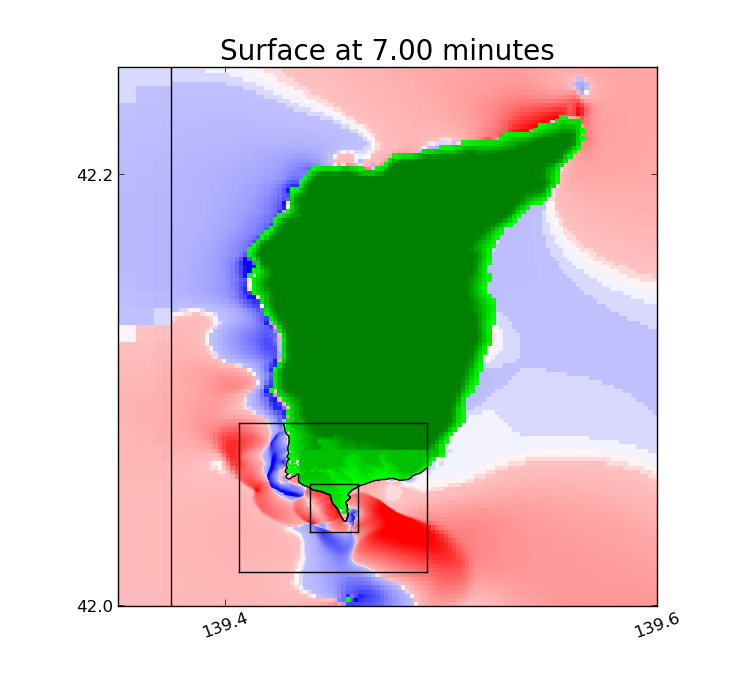
\includegraphics[width=2.0in]{bp9/ok_7min.png}\hfil
\hfil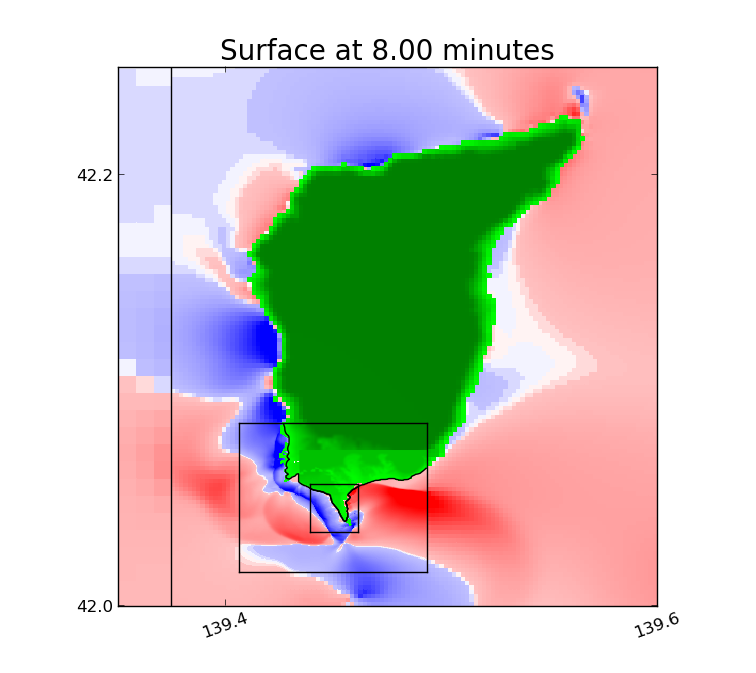
\includegraphics[width=2.0in]{bp9/ok_8min.png}\hfil
\vskip 10pt
\hfil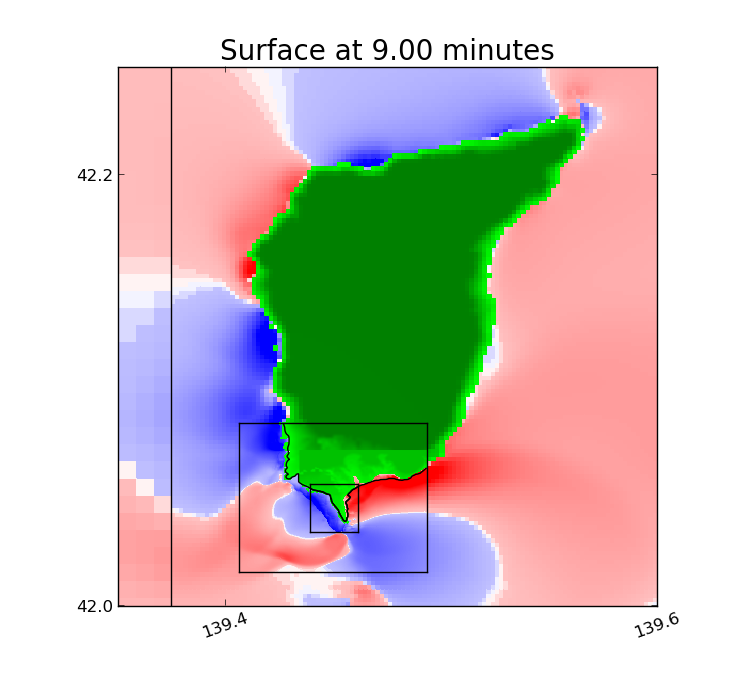
\includegraphics[width=2.0in]{bp9/ok_9min.png}\hfil
\hfil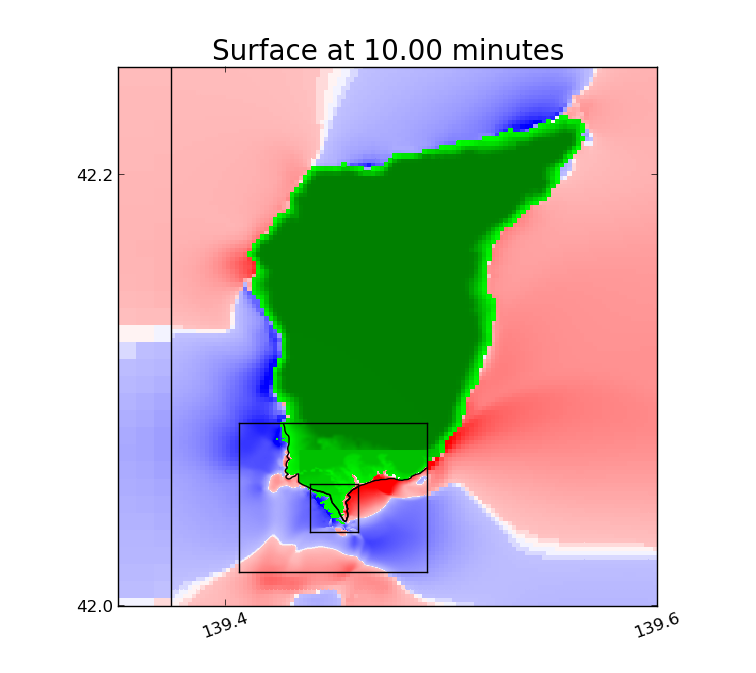
\includegraphics[width=2.0in]{bp9/ok_10min.png}\hfil
\hfil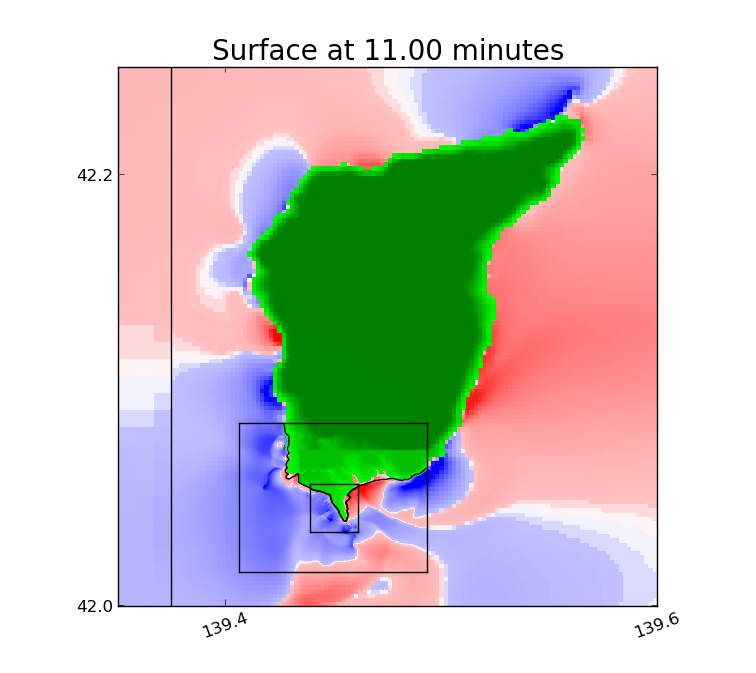
\includegraphics[width=2.0in]{bp9/ok_11min.png}\hfil
\caption{\label{bp9ok}
Zoom on Okushiri Island.
  }
\end{figure}

\begin{figure}[ht]
\hfil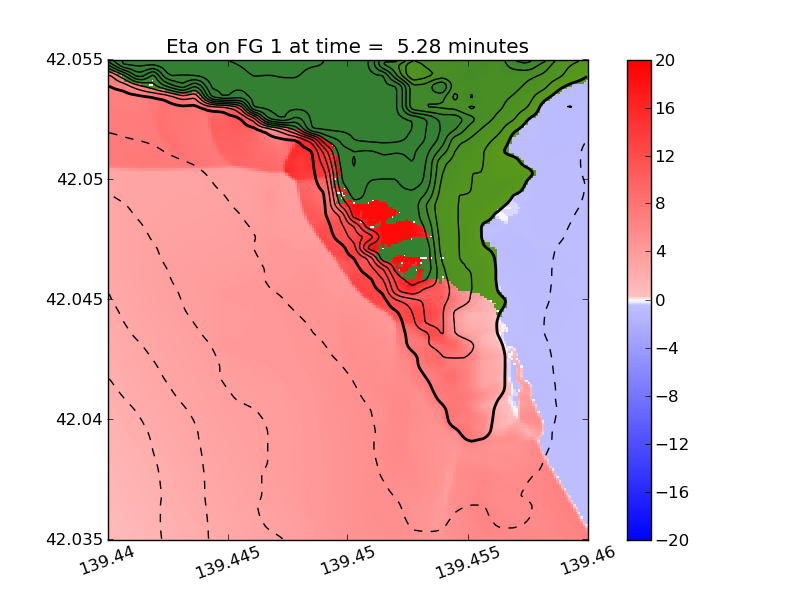
\includegraphics[width=2.8in]{bp9/aonae_5.png}\hfil
\hfil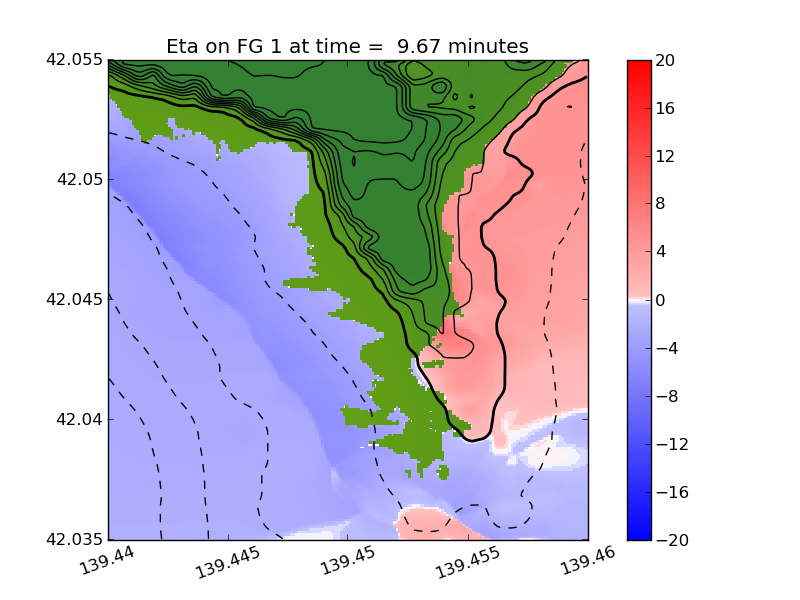
\includegraphics[width=2.8in]{bp9/aonae_14.png}\hfil
\caption{\label{bp9aonae}
Zoom on Aonae Peninsula showing the first wave arriving from the east and the second from the west.  Color map shows elevation of sea surface.  4-meter contours of bathymetry and topography are shown.
  }
\end{figure}

\begin{figure}[ht]
\hfil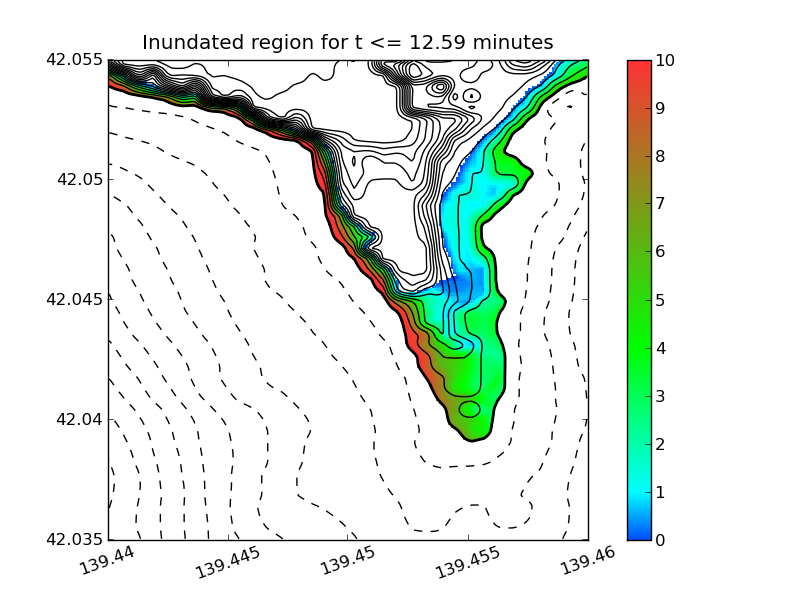
\includegraphics[width=5.0in]{bp9/in_aonae.png}\hfil
\caption{\label{bp9inaonae}
Inundation map of the Aonae Peninsula.  Color map shows maximum fluid depth over entire computation at each point. 4-meter contours of bathymetry and topography are shown. 
  }
\end{figure}

\begin{figure}[ht]
\hfil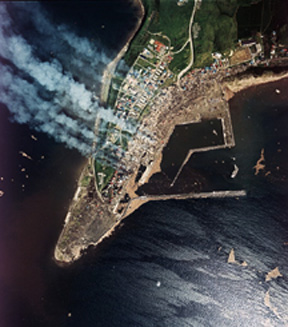
\includegraphics[width=2.8in]{bp9/AonaePhoto.jpg}\hfil
\hfil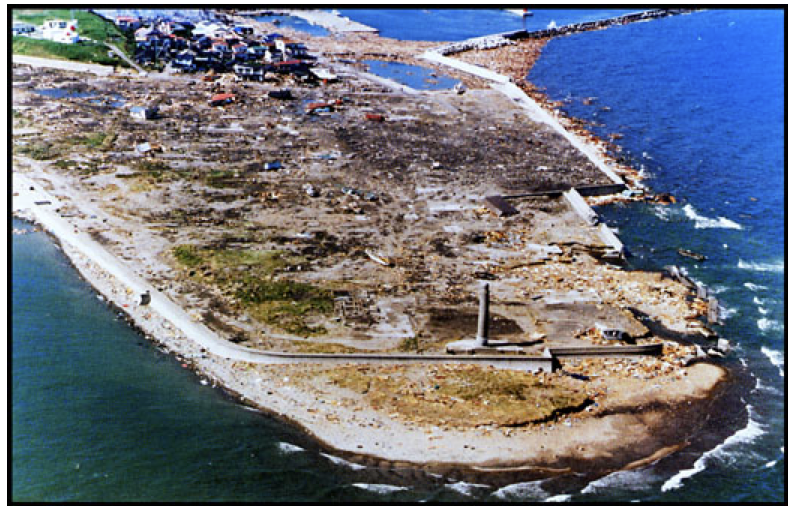
\includegraphics[width=2.8in]{bp9/AonaePhoto2.png}\hfil


\caption{\label{bp9photos}
Photographs of the Aonae Peninsula taken shortly after the event. \\
Left: From \url{http://www.usc.edu/dept/tsunamis/hokkaido/aonae.html}. \\
Right: From \url{http://nctr.pmel.noaa.gov/okushiri_devastation.html}, credited to Y. Tsuji.
  }
\end{figure}

\begin{figure}[ht]
\hfil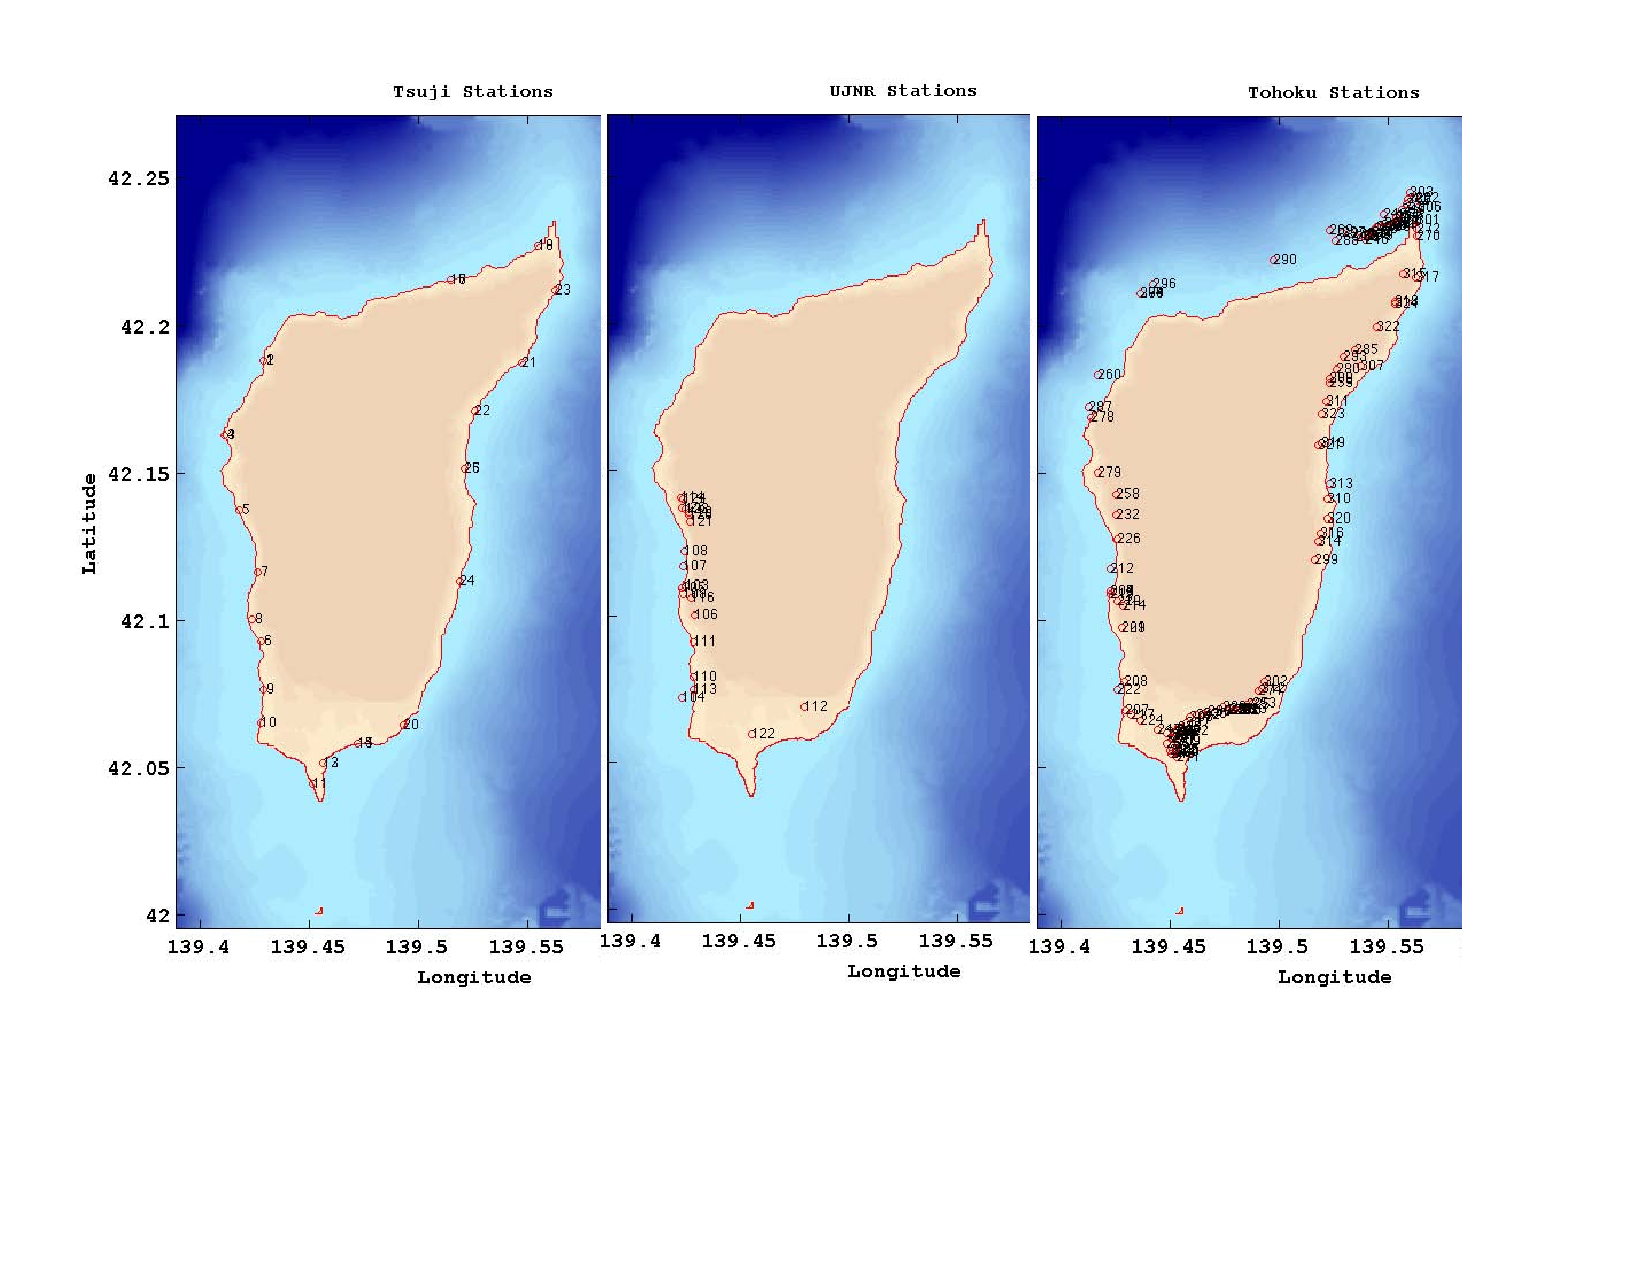
\includegraphics[width=5.0in]{bp9/TeamStations.pdf}\hfil
\vskip 10pt
\hfil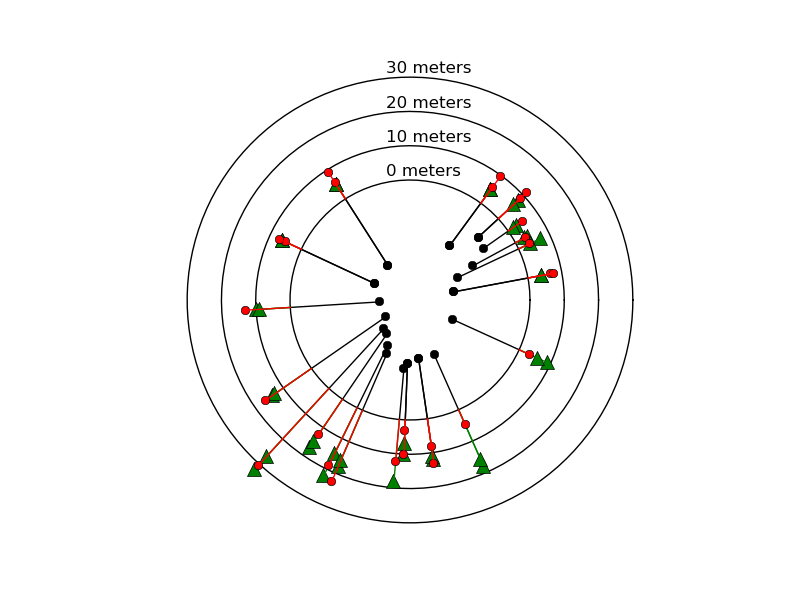
\includegraphics[width=5.0in]{bp9/runups.png}\hfil

\caption{\label{TeamStations}
Top: Locations of field observations by three independent field survey teams, relative to the computational bathy/topo grid system. Only the observations of Tsuji (left figure) were used in this study due to mis-registration of the other two data sets.\\
Bottom: Measured and computed runup at 21 points around Okushiri Island where measured by the Tsuji team.  Red circles are measurements, green diamonds are estimated from the computation.
  }
\end{figure}


% \begin{figure}[ht]
% \hfil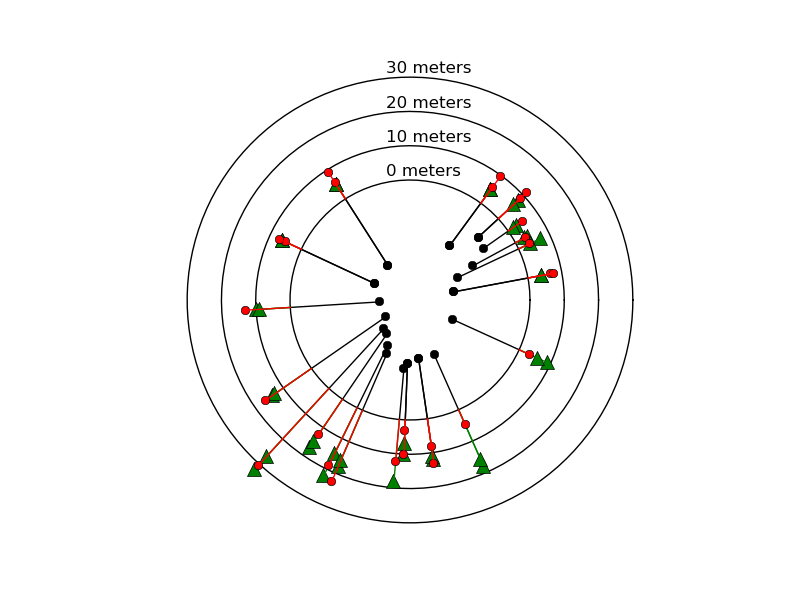
\includegraphics[width=5.0in]{bp9/runups.png}\hfil
% \caption{\label{bp9runups}
% Measured and computed runup at 21 points around Okushiri Island where measured by the Tsuji team.  Red circles are measurements, green diamonds are estimated from the computation.
%   }
% \end{figure}

\begin{figure}[ht]
\hfil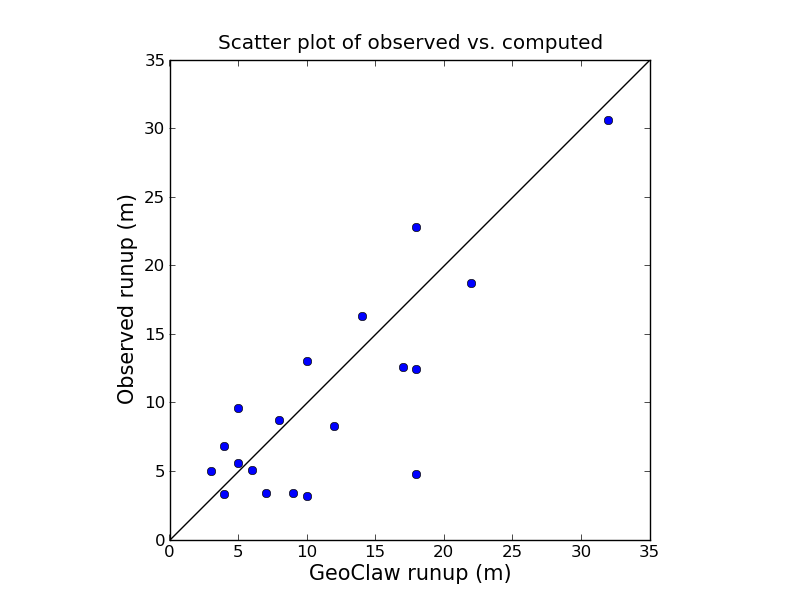
\includegraphics[width=5.0in]{bp9/scatter.png}\hfil
\caption{\label{bp9scatter}
Scatter plot illustrated the correlation between measured and computed values for the values shown in Figure \ref{bp9runups}.
  }
\end{figure}

% \begin{figure}[ht]
% \hfil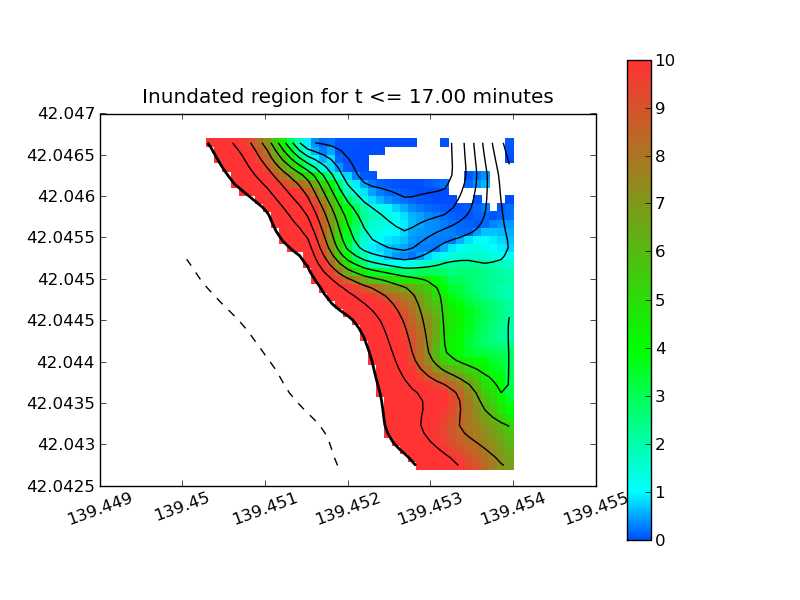
\includegraphics[width=2.8in]{bp9/in_11.png}\hfil
% \hfil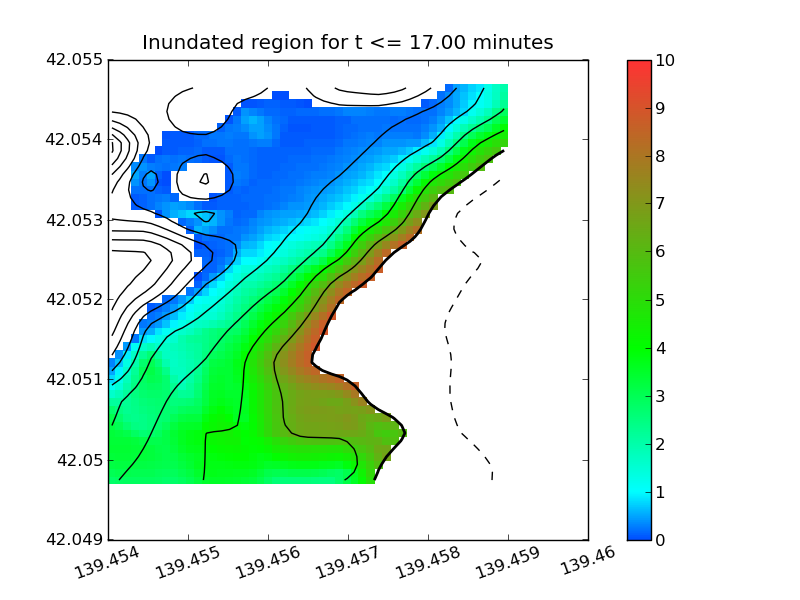
\includegraphics[width=2.8in]{bp9/in_12.png}\hfil
% 
% \caption{\label{bp9fg}
% Sample plots from which runup values are determined.
%   }
% \end{figure}

\begin{figure}[ht]
\hfil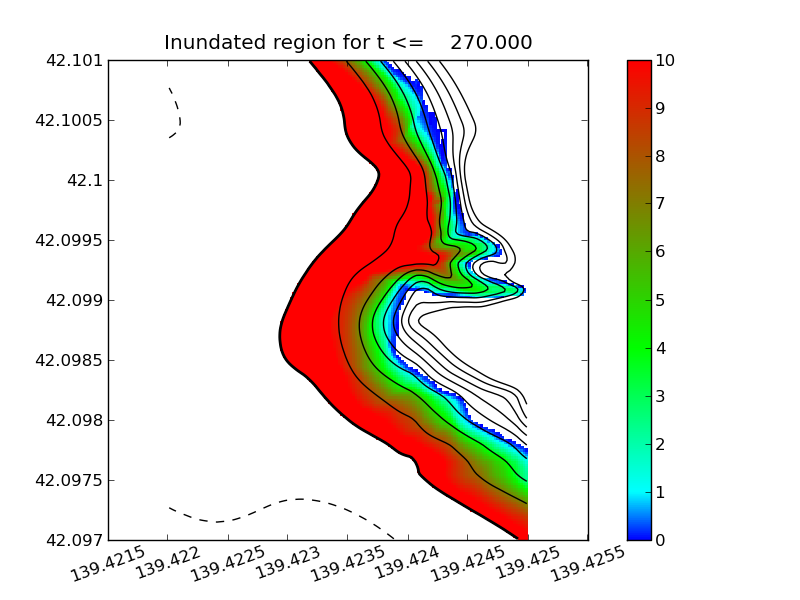
\includegraphics[width=5.0in]{bp9/in_monai.png}\hfil
\caption{\label{bp9monai}
Inundation map of the Monai Valley.  Color map shows maximum fluid depth over entire computation at each point. 4-meter contours of bathymetry and topography are shown. 
  }
\end{figure}

\begin{figure}[ht]
\hfil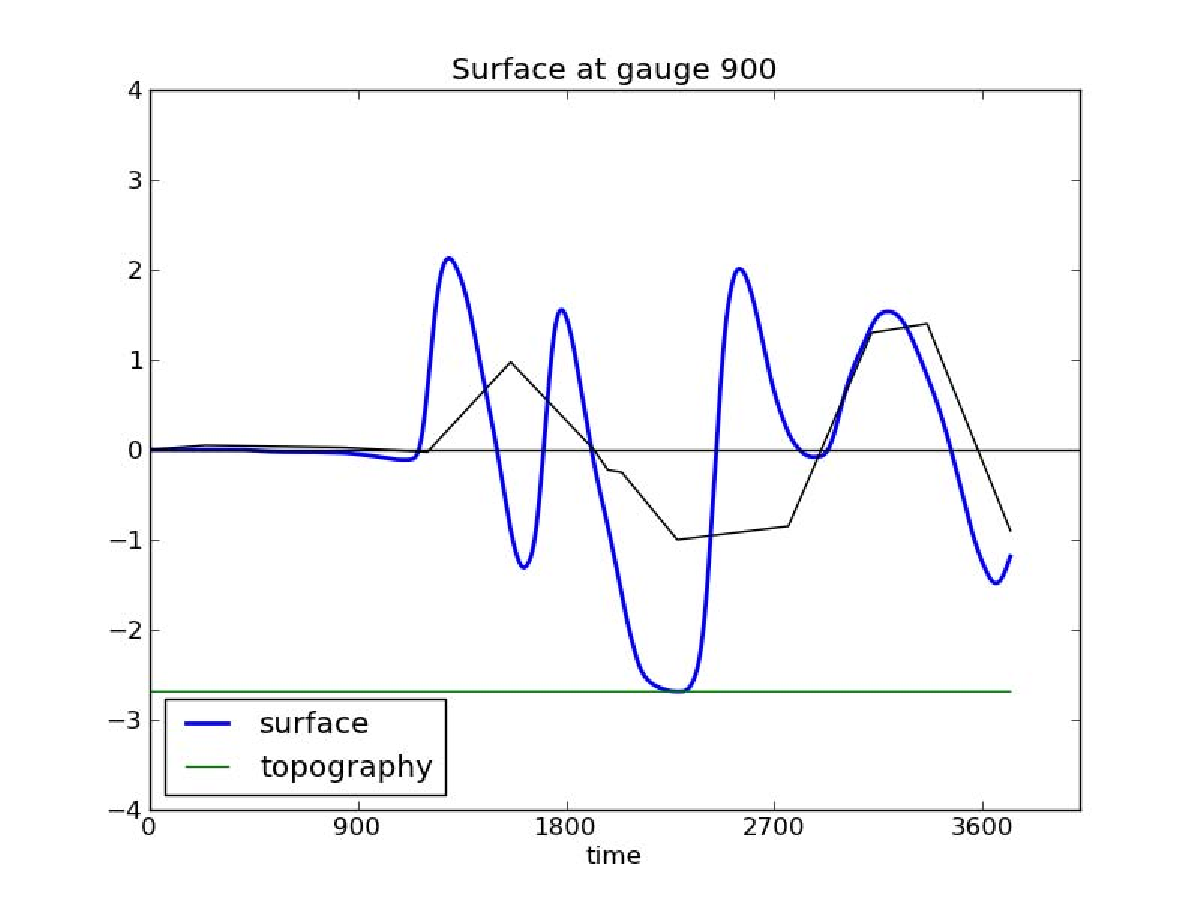
\includegraphics[width=5.0in]{bp9/Iwanai.pdf}\hfil
\caption{\label{Iwanai}
Iwanai tide gage (black line) and GeoClaw (blue line) time series. 
  }
\end{figure}

\begin{figure}[ht]
\hfil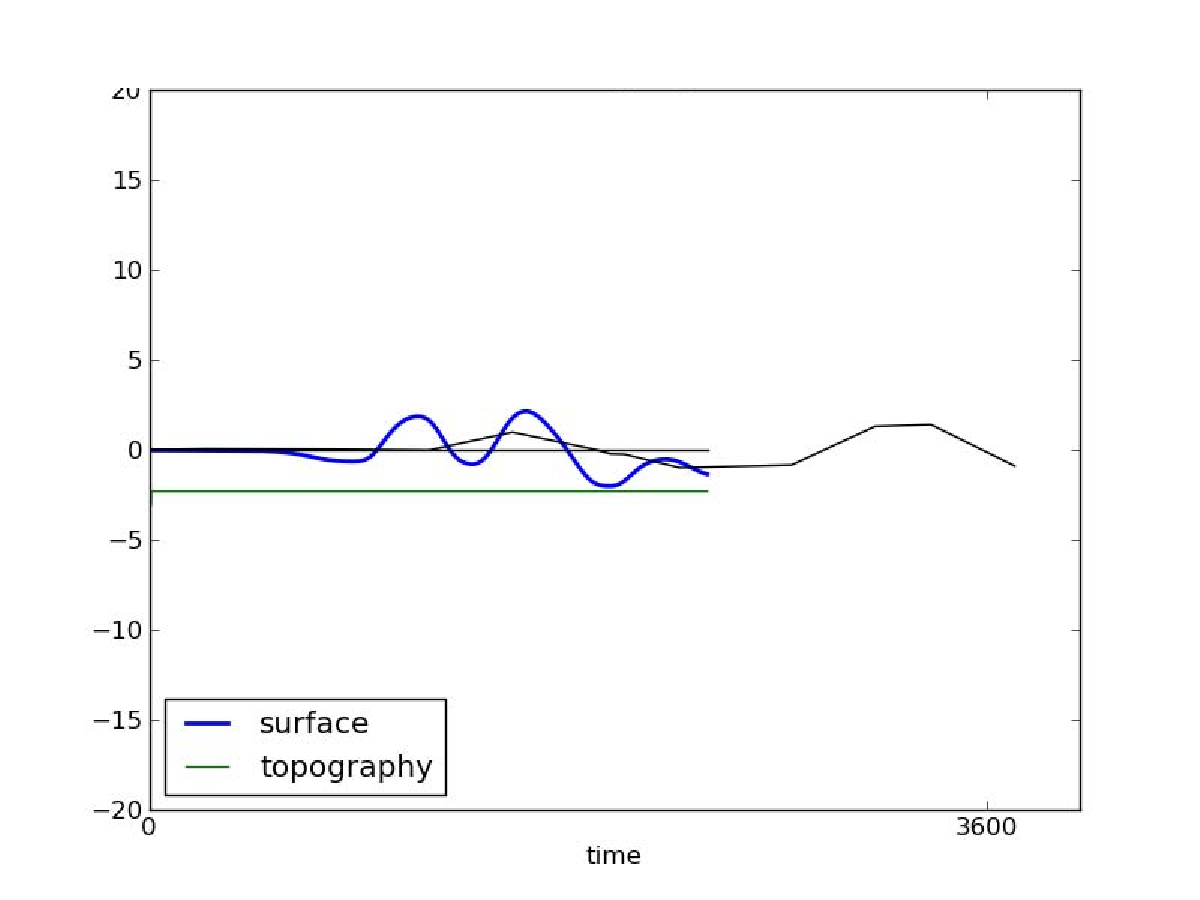
\includegraphics[width=5.0in]{bp9/Esashi.pdf}\hfil
\caption{\label{Esashi}
Esashi tide gage (black line) and GeoClaw (blue line) time series. 
  }
\end{figure}

\subsubsection{Lessons learned}
\begin{itemize}
\item This BenchMark problem requires much more work to qualify as a credible test of tsunami inundation models.  We have little confidence in 
   1. The quality of the bathy/topo computational grids.  A number of mismatches and discontinuities still exist in the system of grids.  A critical related issue is ... 
   2. The accuracy of geospatial registrations of observational and computational latitude and longitude values.  As one example, there appear to be discrepancies in the several field team reports of the latitude and longitude of the highest runup observed, i.e., the value of over 30 m in a `` ... small valley north of Monai ...".  Figure \ref{TeamStations} presents the observation locations of each of three field survey teams -- Professor Yoshinobu Tsuji, Tokyo University (Tsuji), the United States-Japan Cooperative Program on Natural Resources (UJNR) and the Tohoku University (Tohoku) teams.  The bathy/topo computational grids were adjusted to match the positions of the Tsuji observations, but it is clear that this created a systematic error in the registration of the grids with the Tohoku field observations and, in all likelihood, the UJNR field observations.  Such positioning errors can be critical with respect to accurate comparisons of observed and computed runup.
\end{itemize}


\subsubsection{Recommendation}
\begin{itemize}
\item In spite of the currently low quality state of this benchmark problem, the Okushiri tsunami runup and eyewitness observations remains one of the most valuable datasets for model comparisons in existence.  We recommend that an effort be supported to (a) provide a high quality bathy/topo grid system, (b) resolve the ambiguities and discrepancies currently found in the various team data reports to improve the geospatial registration of observed and modeled values, and (c) provide adequate documentation of the resulting benchmark problem dataset.
\end{itemize}



\begin{itemize}
\item 
\end{itemize}
